\section{Zielsetzung und Motivation}
Ziel des Versuches ist es, die spezifische Molwärme von Kupfer in Abhängigkeit der Temperatur zu untersuchen. Die Molwärme C ist die Menge der Wärme, die benötigt wird um ein 1 Mol eines Stoffes um 1 K zu erhitzen. Die  allgemeine Formel  lautet 
\begin{align}
C=\dfrac{\delta Q}{\delta T}
\end{align} 
Außerdem ist zu berücksichtigen, unter welchen Bedingungen die Wärme zu-oder abgeführt wird. Dabei wird unterschieden zwischen der Molwärme bei konstantem Volumen $C_V$ und der Molwärme bei konstantem Druck $C_p$. In diesem Versuch wird die Molwärme $C_V$ gemessen, da sich die Kupferprobe in einem geschlossenen Behältnis mit konstanten Volumen befindet. Desweiteren wird aus den gewonnenen Ergebnissen die sogenannte Debye-Temperatur  $\Theta_D$ bestimmt und mit dem theoretischen Ansatz verglichen. Insgesamt werden drei Modelle untersucht, die die Abhängigkeit der Molwärme von der Temperatur beschreiben. 

\section{Theorie} 
\subsection{Die klassische Theorie der Molwärme}
Die klassische Betrachtung besagt, dass die thermische Energie, die in einen Körper eingebracht wird, sich gleichmäßig auf die Freiheitsgrade der Atome des Festkörpers verteilt. Die Atome sind durch Gitterkräfte an feste Plätze gebunden und können in drei Richtungen schwingen und haben somit drei Freiheitsgrade. Die Atome führen eine harmonische Schwingung um ihre Ruhelage aus und haben somit eine mittlere kinetische Energie, die mit der potentiellen Energie identisch ist. Pro Freiheitsgrad besitzt jedes Atom die Energie $\dfrac{1}{2}k_BT$. Die mittlere Energie eines Atoms ist die Summe der potentiellen und kinetischen Energie und beträgt
\begin{align}
E=6\dfrac{1}{2}k_BT
\end{align}
mit der Boltzmann-Konstante $k_B$  und der Temperatur T. In einem Kristall betrachtet, ergibt sich daraus mit der Loschmidt-Konstante $N_L$ (Teilchendichte eines idealen Gases)
\begin{align}
E=3k_bN_LT.
\end{align}

Unter Vorraussetzung eines konstanten Volumens folgt für die spezifische Wärmekapazität
\begin{align}
C_V=\left(\dfrac{\delta E}{\delta T}\right)_V=3R.
\end{align}
Somit ist die spezifische Molwärme nach der Gleichung (3) material-und temperaturunabhängig. In der Realität trifft diese Annahme nur für hohe Temperaturen ($T\gg\Theta_D$) zu. Bei niedrigen Temperaturen kommt es zu einer sehr starken Abweichung. Zusätzlich zeigt sich in den Messungen, dass die Molwärme materialabhängig ist, was mit der klassischen Theorie nicht übereinstimmt. Die klassische Theorie ist deshalb unzureichend, weil die Quantenmechanik nicht berücksichtigt wird.
\subsection{Die Einstein-Theorie}
Im Einsteinschen-Modell wird im Gegensatz zur klassischen Theorie die Quantelung der Schwingungsenergie der Atome berücksichtigt. Dabei wird angenommen, dass alle Atome im Festkörper jeweils mit der gleichen Frequenz $\omega_E$ schwingen und nur Energien von ganzzahligen Vielfachen des Wertes $\hbar\omega$ aufnehmem bzw. abgeben. Mittels der Boltzmannschen Wahrscheinlichkeitsverteilung 
\begin{align}
W(n)=exp\left(\dfrac{-n\hbar \omega_E}{k_BT}\right)
\end{align}
wird die Wahrscheinlichkeit eines sich im thermischen Gleichgewicht befindenen Oszillators mit der Energie $n\hbar\omega$ bei einer Temperatur $T$ angegeben. Anschließend wird über alle Energien $n \hbar \omega$ von $n=0$ bis $\infty$ multipliziert, mit der Wahrscheinlichkeit $W(n)$ ihres Auftretens summiert und das Ergebnis durch die Summe aller $W(n)$ geteilt. Daraus ergibt sich die Einstein-Energie
\begin{align}
E_{Einstein}=\dfrac{\hbar\omega_E}{e^{\dfrac{\hbar \omega_E}{k_BT}}-1}.
\end{align}
Die Molwärme berechnet sich somit zu 
\begin{align}
C_V=3R\left(\dfrac{\hbar\omega_E}{k_B}\right)^2 \dfrac{1}{T^2} \dfrac{exp\left(\dfrac{\hbar\omega_E}{k_BT}\right)}{\left(exp\left(\dfrac{\hbar \omega_E }{k_BT}\right)-1\right)^2}
\end{align}
mit der Einstein-Temperatur $\Theta_E=\dfrac{\hbar \omega_E}{k_BT}$, die mit der Einstein Frequenz zusammenhängt. Auch bei diesem Modell gilt eine Annäherung an 3R bei sehr hohen Temperaturen. Bei einer Abnahme der Temperatur nimmt die Molwärme ebenfalls ab. Für tiefe Temperaturen zeigt sich, dass der Verlauf der speziellen Molwärme mit der Temperatur exponentiell zunimmt. Auch in diesem Modell tritt für tiefe Temperaturen eine Abweichung zu experimentellen Werten auf aufgrund der Annahme, dass alle Atome mit gleicher Frequenz schwingen. 
\subsection{Debye-Modell}
Eine bessere Annäherung an die  experimentellen Messwerte bietet das Debye-Modell.
Das Modell basiert darauf, dass die Eigenschwingungen aller Oszillatoren in einem Festkörper eine spektrale Frequenzverteilung $Z(\omega)$ mit der  Grenzfrequenz $\omega_D$ besitzt.Ein Kristall besitzt aufgrund endlicher Dimension nur endlich viele Eigenschwingungen. Diese beträgt $ 3 N_L$ , wobei $N_L$ die Loschmidt-Konstante ist und die Anzahl der Moleküle pro Volumen eines idealen Gases angibt. Daher existiert eine Grenzfrequenz $\omega_D$, die auch Debye-Frequenz genannt wird und über die Formel 
\begin{align}
\int_{0}^{\omega_D}Z(\omega)d\omega=3N_L
\end{align}
berechnet wird. Bis zur dieser Grenzfrequenz ist die lineare Dispersionsrelation (Frequenz und Wellenvektor proportional) gegeben. Durch Verknüpfen der klassischen und des quantenmechanischen Modells, ergibt sich eine Näherung mit der Form für die spektrale Verteilung von 
\begin{align}
Z(\omega)d\omega=\dfrac{L^3}{2\pi^2}\omega^2\left(\dfrac{1}{v_{long}^3}+\dfrac{2}{v_{trans}^3}\right)d\omega.
\end{align}
Dabei wird angenommen, dass die Phasengeschwindigkeit einer elastischen Welle nicht von ihrer Frequenz und ihrer Ausbreitungsrichtung abhängt. Sodass $Z(\omega)$ sich berechnen lassen kann durch Abzählen der Eigenschwingungen in einem Würfel mit Kantenlänte $L$. 
Mit der Debye-Grenzfrequenz wird diese Gleichung zu 
\begin{equation}
Z(\omega)d\omega=\dfrac{9N_L}{\omega_D^3}\omega^2 d\omega.
\end{equation}
Die freie Schwingungsenergie berechnet sich über die Formel:
\begin{equation}
U=\int_{0}^{\omega_D}\dfrac{Z(\omega)d\omega}{e^{\dfrac{\hbar \omega}{k_B T}-1}}
\end{equation}
Die Wärmekapazität $C_v$ ergibt durch Ausführung des Integrals und der Differentiation nach der Temperatur. 
\begin{equation}
C_{V,Debye}=\dfrac{d}{dT}\dfrac{9N_L}{\omega_D^3}\int_{0}^{\omega_D}\dfrac{\omega^3}{exp(\hbar\omega/k_BT)-1}
\end{equation}
Wie bei den anderen Modellen, nähert sich auch die Debye Kurve im hohen Temperatur Bereich dem Wert $3R$ an. Und für niedrige Temperaturen ($T\rightarrow 0$) ergibt sich eine $T^3-$Abghängigkeit. 

\subsection{Vergleich der drei Modelle}
In der Abbildung \ref{fig:vergleich} werden die Verläufe der drei Modelle mit dem experimentellem Befund verglichen. Zunächst ist zu erkennen, dass für hohe Temperaturen (ab 300 K) das Einstein- und das Debye Modell sich dem Wert von 3R annähern. Für niedrige Temperaturen (0-300K) hingegen nimmt der Verlauf der speziellen Molwärme nach Einstein exponentiell mit der Temperatur zu, wohingegen es bei dem Debye-Modell eine $T^3$-Abhängikeit für tiefe Temperaturen gibt. Anhand der Abbildung lässt sich erkennen, dass das Debye-Modell sich dem experimentellen Verlauf am meisten nähert. Außerdem ist in der Abbildung der Verlauf der der Wärmekapazität in Abängigkeit der Temperatur für das freie Elektronengas abgebildet. Es erigibt sich eine lineare Abhängigkeit. Es zeigt sich, dass der Beitrag der spezifischen Wärme der Elektronen zur gesamten Wärmekapazität nur in sehr niedrigen Temperaturen($T\rightarrow 0$) eine wichtige Rolle spielt. Wohingegen für höhere Temperaturen der Beitrag nur sehr gering ist. 

\begin{figure}[h!]
	\centering
	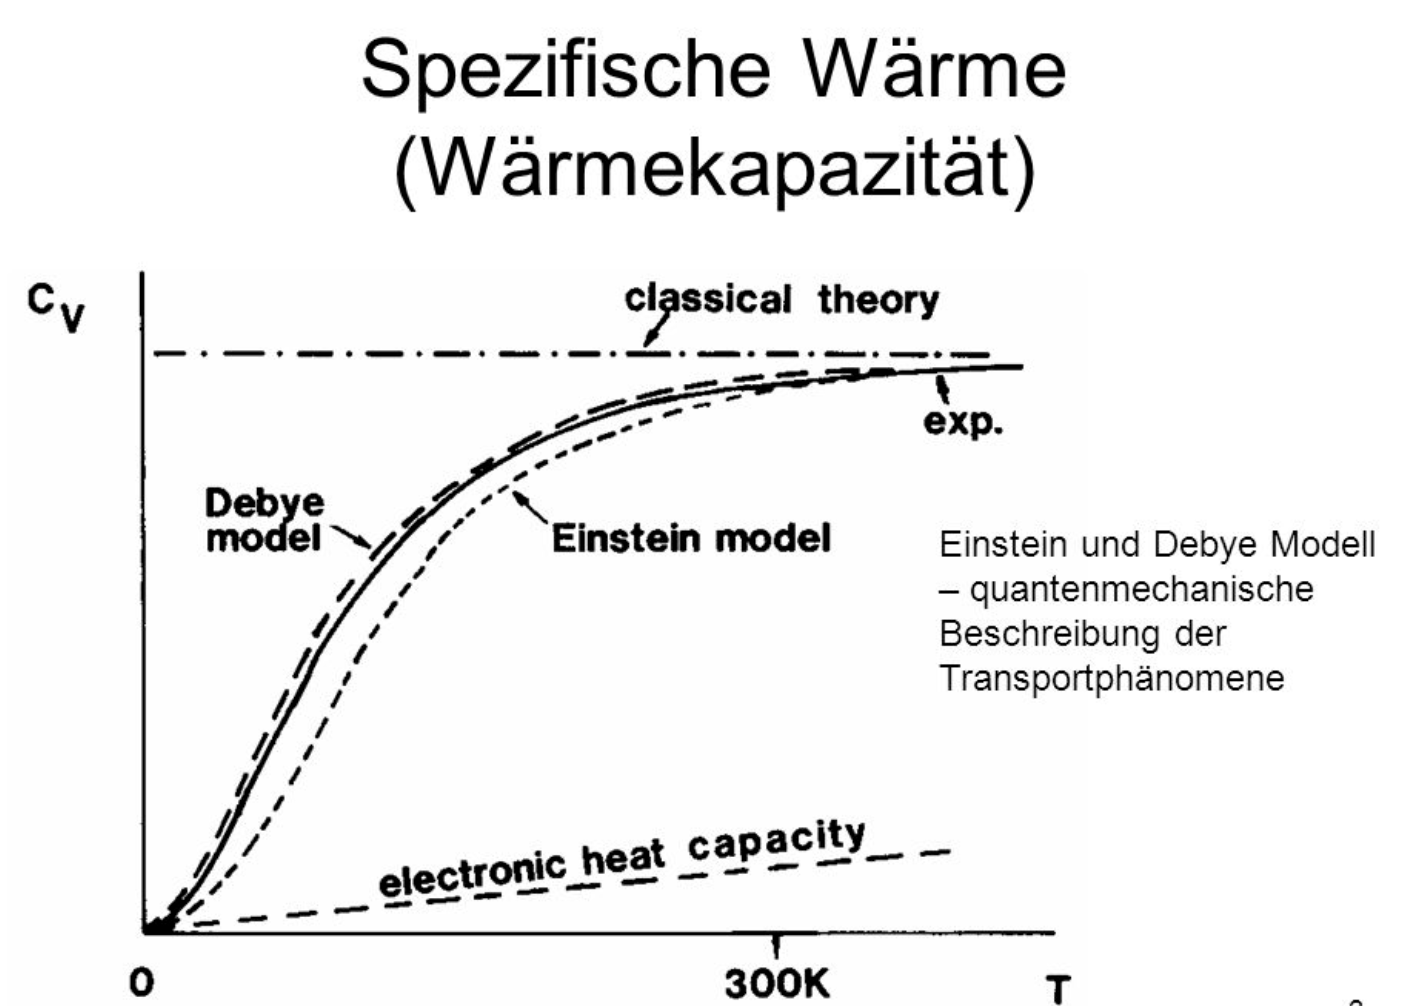
\includegraphics[width=0.7\linewidth]{../vergleich}
	\caption{Vergleich der drei Graphiken von der klassischen Theorie, des Einstein-Modells und des Debye-Modells, \cite{Vergleichder3Modelle}.}
	\label{fig:vergleich}
\end{figure}


